\chapter{Operazioni sui dati e Modellazione relazionale}
\label{cha:Data_op}

\section{Pulizia e Pre Elaborazione dei Dati} \label{par:Pulizia_dati}
% Spiegazione delle scelte fatte sui dati forniti, su queli sono stati ritenuti più importanti

La prima fase operativa del lavoro ha riguardato la \textbf{Selezione e la pulizia dei dati}, con l'obiettivo di ottenere un insieme informativo coerente, affidabile e strettamente correlato alla finalità dello studio.
Partendo dalle informazioni fornite dalle fonti citate nel capitolo precedente \ref{cha:data_prop}, si è proceduto a individuare le variabili ritenute rilevanti per l'analisi, eliminando componenti ridonanti, o potenzialmente non pertinenti. \\

Nel caso del dataset relativo ai passaggi ai tornelli, fornito dalla società \textit{Freccia nel Cielo}, è stato necessario un processo di revisione per assicurare l'integrità e la significatività dei dati. In particolare, è stato riscontrato che il numero totale di passaggi giornalieri (\textbf{Passaggi Tot.}) non corrisponde esattamente alla somma delle tre categorie di skipass  considerate nello studio(Dolomiti Superski, Speciali e Valle).

Tale discrepanza deriva dal fatto che il conteggio totale include anche le \textbf{aperture manuali dei tornelli}, effettuate in casi eccezionali come malfunzionamenti del sistema di lettura o interventi del personale tecnico, nonché i \textbf{passaggi effettuati tramite skipass a punti}.
Questi ultimi rappresentano una quota marginale del totale, poiché lo skipass a punti risulta economicamente conveniente solo su impianti brevi e a basso costo in punti, mentre è poco utilizzato su infrastrutture più lunghe o complesse, come cabinovie e seggiovie principali.

Di conseguenza, la differenza tra il totale dei passaggi e la somma delle tre tipologie di skipass risulta generalmente contenuta, nell’ordine di poche decine di unità giornaliere,  ma è stata comunque ritenuta significativa ai fini della coerenza complessiva del dataset.
Per questo motivo, ai fini dell’analisi, si è scelto di utilizzare il campo \textbf{Passaggi Tot.} come misura di riferimento, poiché rappresenta il valore più completo e comprensivo del traffico effettivo registrato sugli impianti.
Tale scelta consente di garantire una rappresentazione globale dell’affluenza, evitando di sottostimare i volumi complessivi e preservando l’accuratezza delle analisi comparative tra impianti e giornate.
Le misure numeriche dei vari skipass invece, sono state usate prevalentemente in funzione di quale titolo e in che periodo stagionale sia il più popolare all'acquisto. \\


Spostandosi invece sull’elaborazione dei dati meteorologici, si è proceduto a un'attenta selezione delle variabili effettivamente utili ai fini dell’analisi, registrate nella stazione meteorologica di \textbf{Cortina d’Ampezzo – Gilardon}, gestita da ARPA Veneto, che immagazzina dati in modo continuo con  molteplici parametri atmosferici.
Tuttavia, per garantire la coerenza con gli obiettivi dello studio, sono stati esclusi i dati relativi alla radiazione solare, al livello idrometrico e all’umidità relativa, in quanto considerati troppo specifici dal punto di vista tecnico e non direttamente significativi per l’analisi del comportamento turistico e sportivo degli utenti.

Tali misure, pur scientificamente rilevanti, non rientrano tra le informazioni comunemente consultate da uno sciatore o da un visitatore nel processo decisionale quotidiano (ad esempio, la scelta di recarsi o meno sulle piste).
L’obiettivo del presente lavoro è infatti quello di descrivere le correlazioni tra condizioni meteorologiche percepite — quali temperatura, vento e precipitazioni — e i flussi di affluenza agli impianti sciistici, tralasciando le variabili di natura più tecnica o specialistica che non influiscono direttamente sulle dinamiche di utilizzo delle infrastrutture turistiche.\\

Durante la fase di pulizia, è stata inoltre effettuata una normalizzazione dei valori nulli (\textbf{Null}) presenti in alcune variabili, dovuti a momentanee assenze di rilevamento da parte della stazione meteorologica.
In particolare, i campi relativi alla velocità e direzione del vento, visionabili nel loro formato ideale nella Tabella~\ref{tab:rilevamento_dati}, risultavano occasionalmente incompleti, e tali record sono stati esclusi dall’analisi per evitare distorsioni statistiche o interpretative.
L’eliminazione di questi valori ha garantito la consistenza interna del dataset e la comparabilità temporale delle serie di dati utilizzate per le analisi multidimensionali successive.\\

A seguito delle operazioni di pulizia e normalizzazione, l’insieme dei dati risultante è stato ritenuto idoneo per la successiva fase di modellazione relazionale e costruzione dello schema concettuale.





\section{Modello concettuale dei Dati}
% introduzione al modello concettuale 
% spiegazione delle chiavi artificiali introdotte che non sono presenti nei dati (vedi nota : Thesis)

L’organizzazione e la rappresentazione dei dati raccolti si basano su un \textbf{modello relazionale}, costruito a partire dal paradigma Entity–Relationship (E–R), introdotto negli anni Settanta e tuttora ampiamente impiegato nella modellazione concettuale dei dati \cite{ER_Model}.
Questo approccio consente di descrivere in maniera strutturata e formale le entità coinvolte in un dominio applicativo e le relazioni che intercorrono tra di esse, specificandone la cardinalità, le dipendenze logiche e i vincoli di integrità.
Attraverso la modellazione E–R è possibile rappresentare in modo chiaro la struttura concettuale del dominio informativo, costituendo così la base per la successiva progettazione logica e fisica del database e per l’evoluzione verso schemi multidimensionali più complessi impiegati nei sistemi di \textbf{Business Intelligence}. \\

Lo schema di modellazione adottato è quello a Costellazione (Fact Constellation Schema), un’estensione dello schema a stella in cui le dimensioni possono essere condivise tra più tabelle dei fatti. Questo modello presenta una struttura articolata e flessibile, caratterizzata da una o più tabelle dei fatti collegate a un insieme di dimensioni comuni o normalizzate, in modo simile allo schema a fiocco di neve \cite{databricks_Snowflake}, ma con la peculiarità di supportare più fatti.

Nel contesto di questo lavoro, la scelta della costellazione è motivata dalla necessità di rappresentare il fenomeno osservato a diversi livelli di granularità temporale: sono infatti presenti due tabelle dei fatti, una con dati giornalieri e una con dati stagionali. 

la presenza di due tabelle dei fatti risponde a una precisa esigenza di modellazione e ottimizzazione dell’analisi dei dati.
In un’architettura a costellazione infatti, l’organizzazione dei dati è pensata per consentire interrogazioni analitiche flessibili e ad alte prestazioni, riducendo al contempo ridondanze e ambiguità semantiche. La separazione in due tabelle dei fatti permette di rappresentare in maniera distinta fenomeni informativi di natura diversa ma strettamente correlati: da un lato i dati relativi all’affluenza giornaliera agli impianti sciistici, dall’altro le misure aggregate o stagionali che descrivono l’andamento complessivo nel periodo di osservazione.\\

Questa distinzione garantisce un duplice vantaggio. Da un punto di vista concettuale, consente di differenziare le granularità temporali e operative: la tabella dei fatti giornaliera registra eventi atomici e di breve periodo (es. passaggi giornalieri per impianto e tipologia di skipass), mentre la tabella dei fatti stagionale sintetizza informazioni di più alto livello (es. volumi aggregati per impianto e stagione). Da un punto di vista analitico e prestazionale, la separazione tra le due granularità riduce la complessità delle interrogazioni, semplifica i processi di aggregazione e permette di effettuare analisi comparative e temporali (es. confronti tra stagioni diverse) in modo più efficiente e strutturato.\\


Le componenti strutturali della costellazione, ovvero le \textbf{Tabelle dei Fatti} e le \textbf{Tabelle Dimensionali}, hanno quindi un contenuto differente tra loro.

Le Tabelle dei Fatti rappresentano il fulcro del modello: contengono le misure quantitative oggetto di analisi e le chiavi esterne che le collegano alle dimensioni. 
Un esempio di misura quantitativa, presente nella tabella dei fatti giornalieri nel modello proposto, è il numero totale di passaggi ai tornelli registrato in una singola giornata\footnote{Questa misura costituisce la base per l’aggregazione e l’analisi multidimensionale dei dati operativi.}.\\

Le Tabelle Dimensionali invece, contengono gli attributi descrittivi secondo i quali vengono aggregate e filtrate le misure, come meteo, geografia, prodotto o tipologia di servizio. Nello schema a fiocco di neve, e analogamente in quello a costellazione in quanto sua estensione, le dimensioni possono essere normalizzate, mediante la creazione di sottodimensioni, ovvero tabelle che rappresentano attributi gerarchicamente correlati, riducendo la ridondanza informativa e migliorando la rappresentazione semantica dei dati.\\

Un caso tipico di dimensione normalizzata è rappresentato dalle \textbf{gerarchie temporali}, che permettono di navigare e aggregare i dati secondo diversi livelli di dettaglio temporale. Nel presente modello, la dimensione tempo può essere strutturata gerarchicamente partendo dal giorno e progredendo verso la settimana, il mese e l’anno. Ogni livello gerarchico può essere rappresentato in una tabella distinta oppure mediante attributi multipli all’interno di un’unica tabella dimensionale. Tale struttura abilita operazioni OLAP lungo la dimensione temporale, come drill-down (analisi a un livello di dettaglio maggiore) e roll-up (aggregazione a un livello superiore), migliorando significativamente le capacità di esplorazione e di ricerca di informazioni nel sistema.\\






%descrizione delle entità e relazioni



\section{Fact Constellation Schema}

La seguente sezione illustra nel dettaglio il modello logico implementato secondo lo schema a \textbf{costellazione dei fatti}, derivato dal modello concettuale descritto nella sezione precedente. Tale schema rappresenta la base operativa per la successiva fase di analisi multidimensionale e di costruzione delle visualizzazioni su vatie tematiche di ricerca, consentendo di integrare le informazioni provenienti dalle diverse fonti citate e avendo diversi livelli di dettaglio temporale e dimensionale in un'unica struttura coerente\footnote{La legenda e il modello relazionale sono stati realizzati con \textbf{LucidChart} \cite{Lucidchart}}.\\

\begin{figure}[h]
    \centering
    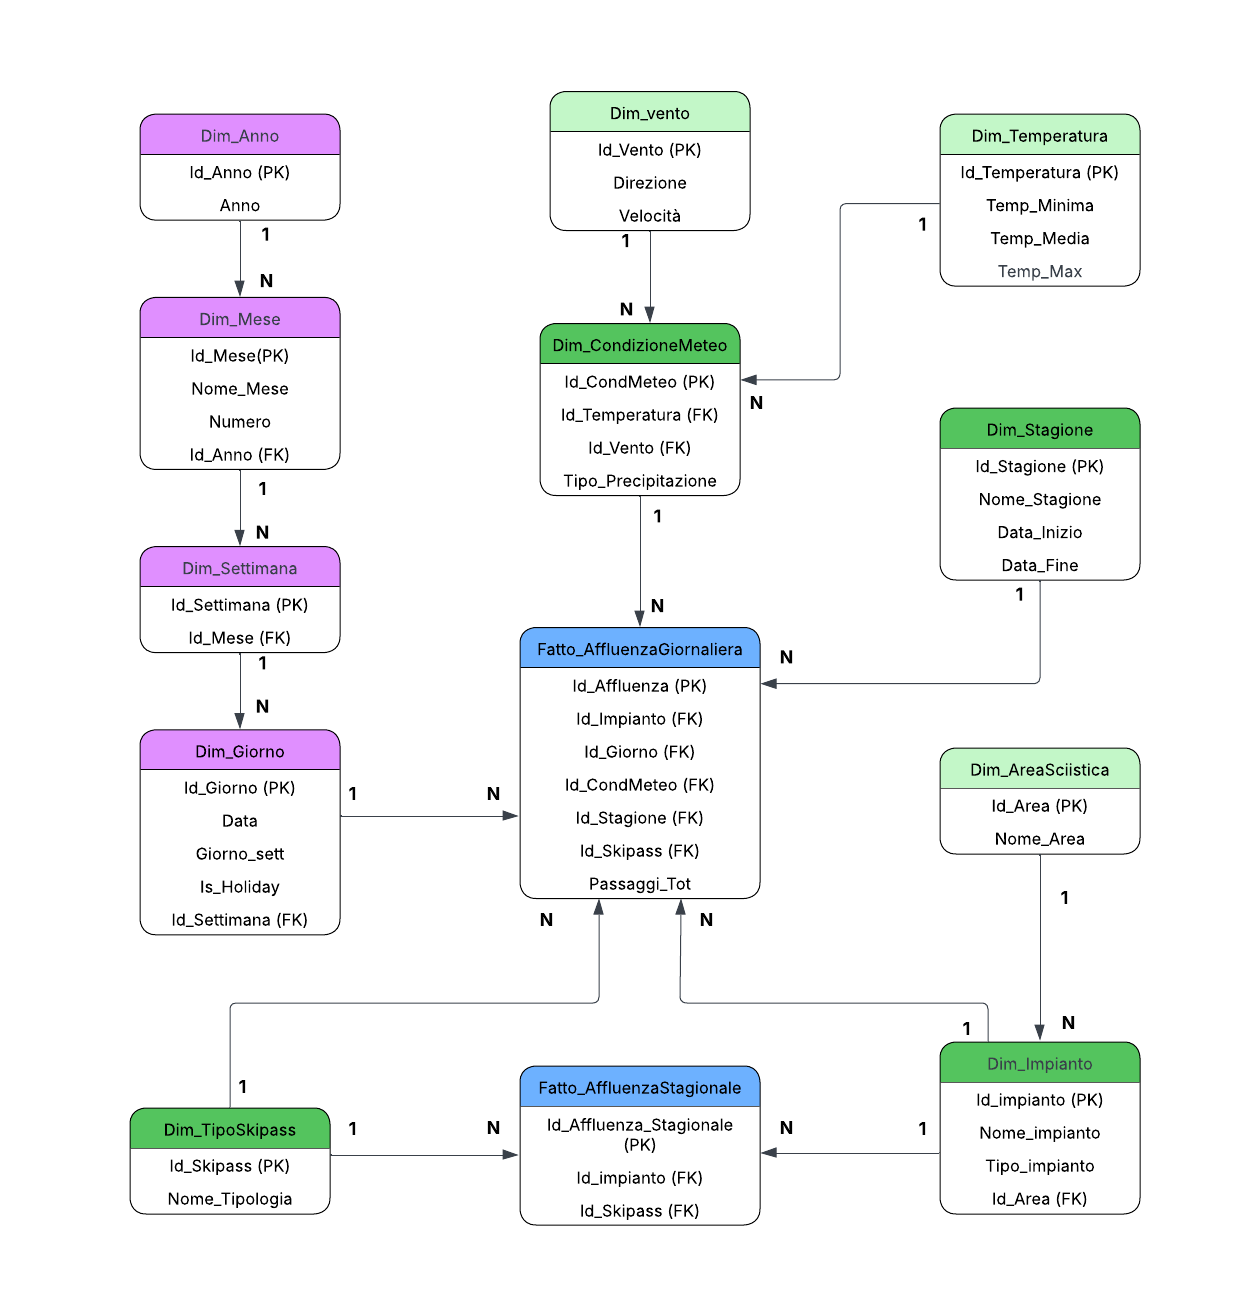
\includegraphics[width=0.9\textwidth]{images/Modello_relazionale/Constellation_Schema.png}
    \caption{Schema logico a costellazione dei fatti del dominio di analisi.}
    \label{fig:fact_constellation}
\end{figure}



\noindent
\textbf{Legenda e convenzioni dello schema.}  
Nello schema logico riportato in Figura~\ref{fig:fact_constellation}, le sigle \textbf{PK} e \textbf{FK} indicano rispettivamente le Primary Key (chiavi primarie) e le Foreign Key (chiavi esterne) delle tabelle.  
Le chiavi primarie identificano in modo univoco ciascun record all’interno della tabella, mentre le chiavi esterne stabiliscono le relazioni con le altre entità del modello, garantendo l’integrità referenziale del database.
La \textbf{cardinalità} delle relazione è sempre \textbf{1-N} nella direzione delle tabelle dei fatti, come da convezione per lo schema a costellazione.\\

È opportuno precisare che le chiavi primarie non erano presenti nei dataset originali forniti dalle aziende, ma sono state introdotte artificialmente durante la fase di progettazione logica per consentire un’identificazione univoca dei record e assicurare la coerenza del modello relazionale.  
Questa scelta è comune nella modellazione concettuale dei dati e rappresenta una buona pratica per la costruzione di schemi complessi come quelli multidimensionali.\\


Inoltre le etichette delle tabelle dei fatti e dimensionali hanno colorazioni per evidenziarne le differenze seguono la legenda sottostante \ref{fig:uml_legend}.

\begin{figure}[h]
    \centering
    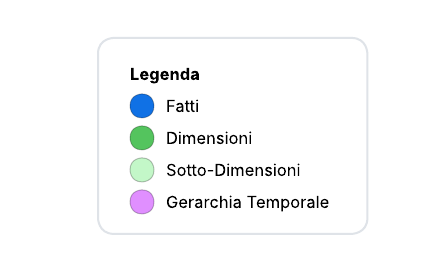
\includegraphics[width=0.4\textwidth]{images/Modello_relazionale/Legenda_Schema.png}
    \caption{Legenda UML adottata nello schema logico}
    \label{fig:uml_legend}
\end{figure}

La comprensione delle convenzioni grafiche e delle chiavi utilizzate consente ora di analizzare nel dettaglio la struttura del modello, a partire dalle \textbf{Tabelle dei Fatti}, che costituiscono il nucleo centrale della costellazione, per poi proseguire con la descrizione delle \textbf{Tabelle Dimensionali} e delle rispettive gerarchie di riferimento.\\

\subsection{Tabelle dei Fatti}

Il modello, come illustrato nel capitolo precedente, si articola attorno a due fatti principali, \textbf{Fatto\_AffluenzaGiornaliera} e \textbf{Fatto\_AffluenzaStagionale}, che  rendono necessario l'impiego di uno schema a costellazione.
Questra struttura consente di rappresentare il fenomeno dell'affluenza turistica con granularità temporali differenti (giornaliera e stagionale), mantenendo la coerenza delle relazioni tra le dimensioni e garantendo una visione integrata del dominio analizzato.


\paragraph{Fatto\_AffluenzaGiornaliera}
Rappresenta il cuore del modello dal punto di vista operativo, registrando i dati elementari relativi all'affluenza quotidiana sulle piste da sci.
Ogni record descrive un evento giornaliero, identificato da un insieme di chiavi esterne che consentono di recuperare i record correlati nelle varie dimensioni:
\textbf{Id\_Giorno}, \textbf{Id\_Impianto}, \textbf{Id\_Skipass}, \textbf{Id\_CondMeteo} e \textbf{Id\_Stagione}.
La misura quantitativa principale è rappresentata da \textbf{Passaggi\_Tot}, che indica il numero complessivo di passaggi ai tornelli degli skipass avvenuti in quella specifica giornata.
Questa tabella consente analisi ad alta risoluzione temporale e confronti mirati tra impianti, giornate e condizioni meteorologiche, fornendo una base di dettaglio per successive aggregazioni stagionali.

\paragraph{Fatto\_AffluenzaStagionale}
La seconda tabella dei fatti contiene dati aggregati su base stagionale, ottenuti tramite operazioni di sintesi (roll-up) sulla tabella giornaliera.
Le sue chiavi esterne principali (\textbf{Id\_Impianto}, \textbf{Id\_SKipass}, \textbf{Id\_Stagione}) riflettono la struttura comune condivisa con la tabella giornaliera, consentendo l'integrazione tra i due livelli di granularità temporale.
Le misure in essa contenute descrivono i volumi complessivi di passaggi e altri indicatori aggregati relativi all'intera stagione sciistica, permettendo lo studio comparativo su scala pluristagionale e l'analisi di trend evolutivi nel tempo.

\subsection{Tabelle Dimensionali}

Le tabelle dimensionali forniscono il contesto descrittivo necessario per interpretare correttamente le misure quantitative.
Nel modello a costelazione, tali dimensioni possono essere condivise da più fatti riducendo la ridondanza dei dati, migliorando la chiarezza semantica e la coerenza logica dell'intero schema. 

\paragraph{Dimensioni temporali}
Il dominio temporale è strutturato secondo più livelli gerarchici per supportare le operazioni OLAP di aggregazione e disaggregazione:

\begin{itemize}
    \item \textbf{Dim\_Giorno}: rappresenta il livello di dettaglio maggiore nella gerarchia; contiene attributi quali la data, il nome del giorno settimanale e un indicatore di festività (Is\_Holiday).
    \item \textbf{Dim\_Settimana}: collega i giorni ai rispettivi intervalli settimanali, fondamentale per valutare l'affluenza nei periodi di alta stagione.
    \item \textbf{Dim\_Mese} e \textbf{Dim\_Anno}: rappresentano i livelli superiori di aggregazione, permettono la maggiore comprensione dei cicli stagionali e delle variazioni di affluenza nel lungo periodo.
\end{itemize}

\paragraph{Dim\_Impianto}
Descrive le caratteristiche strutturali e operative di ciascun impianto di risalita\footnote{Nel modello, anche i passaggi al parcheggio della Freccia nel Cielo vengono trattati come un impianto, al fine di uniformare la struttura analitica}. Gli attributi principali includono \textbf{Nome\_Impianto} e \textbf{Tipo\_Impianto} (es. funivia, cabinovia, seggiovia, ecc.).
Ogni impianto  è inoltre associato a un'area sciistica mediante una relazione di cardinalità \textbf{1-N} con la dimensione \textbf{Dim\_AreaSciistica}, che consente, in prospettiva futura, di ampliare l’analisi a ulteriori comprensori sciistici di Cortina o di altre località dolomitiche, permettendo l’aggregazione per aree geografiche omogenee.

\paragraph{Dim\_TipoSkipass}
Contiene le informazioni relative alle diverse tipologie di Skipass 
che passano al tornello ( es. Dolomiti Superski, Di valle, Agevolati).
Questa dimensione consente di analizzare l'affluenza in relazione al tipo di titolo di accesso, offrend un punto di vista gestionale e commerciale utile alla definizione di strategie tariffarie e politiche di vendita.

\paragraph{Dim\_Stagione}
Fornisce le informazioni descrittive relative alle stagioni invernali comprese nel periodo di osservazione.
Include attributi quali il nome della stagione, la data di inizio e la data di fine, permettendo di aggregare e confrontare le performance stagionali su base cronologica.
La dimensione è strettamente collegata alla tabella dei fatti stagionale, di cui costituisce la chiave logica di riferimento temporale.

\paragraph{Dim\_CondizioneMeteo, Dim\_Temperatura e Dim\_Vento}
Queste tre dimensioni sono utilizzate per descrivere le condizioni atmosferiche prevalenti in una giornata, che influenzano in modo diretto i flussi di affluenza.
\textbf{Dim\_Temperatura} contiene i valori di temperatura minima, media e massima registrati nella giornata.
\textbf{Dim\_Vento} contiene le misurazioni della velocità e direzione del vento.\\

\textbf{Dim\_CondizioneMeteo} integra le precedenti sottodimensioni attraverso le relative chiavi esterne, aggiungendo un attributo relativo al tipo di precipitazione (pioggia, neve o assenza di fenomeni).
Queste dimensioni consentono un’analisi multidimensionale che combina variabili meteorologiche e comportamentali, evidenziando la correlazione tra condizioni climatiche e livelli di affluenza giornaliera.

In sintesi, il modello a costellazione sviluppato integra in modo coerente le diverse dimensioni del dominio: temporale, geografica, meteorologica e gestionale; in un unico sistema analitico, garantendo la precisione dell’analisi giornaliera e la completezza delle valutazioni stagionali.
Tale architettura costituisce la base logica per le successive fasi di visualizzazione e interpretazione dei dati, presentate nel capitolo dedicato alle dashboard analitiche.\\


Per completezza, si riporta in Appendice \ref{appendix:sql} lo script SQL contenente la definizione fisica del database e un esempio di popolamento dei dati, utile per la riproduzione e la verifica del modello relazionale sviluppato.

